\documentclass{beamer}

% Presentation for Kx systems meetup Fall 2016


\mode<presentation>
{
  \usetheme{default}      
  \usecolortheme{default} 
  \usefonttheme{default}  
  \setbeamertemplate{navigation symbols}{}
  \setbeamertemplate{caption}[numbered]
} 

\usepackage{todonotes}
\let\todox\todo
\renewcommand\todo[1]{\todox[inline]{#1}}


\usepackage[english]{babel}
\usepackage[utf8x]{inputenc}
\usepackage{listings}
\usepackage{booktabs}
\usepackage{hyperref}
\hypersetup{
    colorlinks=true,      
    linkcolor=blue,          
    citecolor=blue,        
    urlcolor=blue          
}

\usepackage{tcolorbox}
\usepackage{tikz}
\usepackage{syntax}

% Tikz drawing for architecture and parallel query diagrams
\newcommand{\aquerytikz}{
\tikzstyle{every pin edge}=[<-,shorten <=1pt]
\tikzstyle{elem}=[circle,fill=black!25,minimum size=17pt,inner sep=1pt]
    
\tikzstyle{super-master}=[elem, fill=green!50];
\tikzstyle{master}=[elem, fill=yellow!50];
\tikzstyle{worker}=[elem, fill=blue!50];
}


\lstset{ %
  backgroundcolor=\color{white},   % choose the background color; you must add \usepackage{color} or \usepackage{xcolor}
  basicstyle=\footnotesize,        % the size of the fonts that are used for the code
  breakatwhitespace=false,         % sets if automatic breaks should only happen at whitespace
  breaklines=true,                 % sets automatic line breaking
  captionpos=b,                    % sets the caption-position to bottom
  commentstyle=\color{green},    % comment style
  deletekeywords={...},            % if you want to delete keywords from the given language
  escapeinside={\%*}{*)},          % if you want to add LaTeX within your code
  extendedchars=true,              % lets you use non-ASCII characters; for 8-bits encodings only, does not work with UTF-8
  frame=single,	                   % adds a frame around the code
  keepspaces=true,                 % keeps spaces in text, useful for keeping indentation of code (possibly needs columns=flexible)
  keywordstyle=\color{blue},       % keyword style
  language=Octave,                 % the language of the code
  otherkeywords={*,...,of, on, at, buy, sell, shares},           % if you want to add more keywords to the set
  numbers=left,                    % where to put the line-numbers; possible values are (none, left, right)
  numbersep=5pt,                   % how far the line-numbers are from the code
  numberstyle=\tiny\color{gray}, % the style that is used for the line-numbers
  rulecolor=\color{black},         % if not set, the frame-color may be changed on line-breaks within not-black text (e.g. comments (green here))
  showspaces=false,                % show spaces everywhere adding particular underscores; it overrides 'showstringspaces'
  showstringspaces=false,          % underline spaces within strings only
  showtabs=false,                  % show tabs within strings adding particular underscores
  stepnumber=2,                    % the step between two line-numbers. If it's 1, each line will be numbered
  stringstyle=\color{pink},     % string literal style
  tabsize=2,	                   % sets default tabsize to 2 spaces
  title=\lstname ,                  % show the filename of files included with \lstinputlisting; also try caption instead of title
  upquote=true
}


% Caption stuff
\setbeamerfont{caption}{size=\footnotesize}
\setlength\abovecaptionskip{-5pt}
% Figure paths
\graphicspath{{./figures/}}

\title[orderly]{Orderly: A Tutorial for PL development targeting q/kdb+}
\author{Dennis Shasha and Jos\'e Pablo Cambronero}
\institute{Courant Institute/New York University}
\date{\today}

\begin{document}

\begin{frame}
  \titlepage
\end{frame}

\section{Introduction}

\begin{frame}{Motivation}
Why would we want our own PL?
	\begin{itemize}
  		\item Design freedom
		    	\begin{itemize}
				\item syntactic
				\item semantic
			\end{itemize}
		\item Fit the language to the task (rise in popularity of DSLs)
		\item Enable custom optimizations
  		\item \todo{ more here }
	\end{itemize}
	
Why do we want to target q/kdb+?
	\begin{itemize}
		\item High level
		\item Easy meta programming (parse/eval): $data \leftrightarrow program$
		\item Blazing fast (something everyone in this room knows)
	\end{itemize}	
\end{frame}

\begin{frame}{Two Popular Approaches for DSLs: Internal vs External}
\begin{itemize}
	\item Internal: interpreter embedded in q
		\begin{itemize}
			\item shallow
			\item deep
		\end{itemize}
	\item External: "compiler" (translator) external to q (AQuery)
	\item Both have pros and cons
	\item Internal pros: can take advantage of all language constructs, can take advantage of runtime information
	\item External pros: rewrites can be performed statically (sometimes), can generate transparent code available to user
\end{itemize}
\end{frame}

\begin{frame}{Overview of DSL Approaches}
	\begin{itemize}
		\item Some of these definitions are not clear cut, and authors vary but general idea is:
		\item External: stand-alone, with own parser, (possibly analysis), translation, and execution \cite{artho}
		\item Internal (aka embedded): extend an existing language
			\begin{itemize}
				\item Shallow: DSL implemented directly in the host language semantics, using function calls (no AST built)
				\item Depp: Constructs AST through calls, semantics are given by an "interpreter" function\cite{gibbons}
				\item There are some very interesting, and deeper connections, between the two initially disparate-seeming approaches, see \cite{gibbons} for a nice overview
	\end{itemize}
		\item AQuery: a hybrid between external and internal. Has standalone parsing and translation, but relies on q for execution and allows embedding of literal q code in AQuery files
	\end{itemize}
\end{frame}

\begin{frame}{Orderly: A (very simple) DSL for market orders}
	\begin{itemize}
		\item We need a language simple enough to address in 20-30 min but meaty enough for fun (or at least stave off boredom)
		\item Viol\`a: Thus Orderly was born, a simple DSL to express market orders and insert them into some main order book
		\item We'll follow two approaches:
			\begin{itemize}
				\item "External": Standalone parsing, analysis and translation in \href{https://github.com/josepablocam/kxmeetup/tree/master/orderly-external}{external-orderly}
				\item "Internal (deep)": Parsing using \lstinline{o)} mode, analysis and execution in \href{https://github.com/josepablocam/kxmeetup/tree/master/orderly-internal}{internal-orderly}
			\end{itemize}
	\end{itemize}
\end{frame}

\begin{frame}[fragile]{Orderly BNF}
	\begin{grammar}
		<program> ::= (<order> "->" <ident>) +

		<order>  ::= <side> <vol> "of" <ident> "at" <num> <modifier> ("for" <ident>)?

		<side> ::= "buy"  \alt "sell"

		<vol> ::= <num> "shares" \alt "\$" <num>

		<mod> ::= "if" "\""<monadic-fun-in-q>"\"" \alt "on" <date>
	\end{grammar}
\end{frame}

\begin{frame}[fragile]{Orderly Examples}
\begin{lstlisting}[language=C]
 sell 1000 shares of IBM at $50 on 05/16/2016 for BAML -> order_book
  // uses an embedded q fun
 buy $1e6 of AAPL at $100 if "{[env] 10 < first exec avg close_price from env where sector=Tech} " -> order_book
\end{lstlisting}
\end{frame}


%\begin{frame}{Jose's notes for how the presentation would go:}
%\begin{enumerate}
%\item It is structured around 3/4 main stages of the development process (syntax analysis, semantic analysis, optimization, code generation/execution)
%\item In each slide I would plan to provide some context of what the task is, how to address it if you choose to go with an embedded language vs an external language (I will have written up code for both, and make it available after/during talk...but I prefer not to code live....to easy to make mistakes and distract from presentation goals)
%\item Add videos/screenshots of the task done in the two possible versions (embedded vs external)
%\item For each slide, provide dos/donts
%\item  Discuss briefly how this went into AQuery and how it is done there
%\end{enumerate}
%\end{frame}


\begin{frame}{Syntax Analysis (aka tokenization + parsing) }
\begin{itemize}
	\item We won't dwell on this point
	\item Main takeaway: generate useful parser errors (with context and/or source location if possible)
	\item Ideally parsing code is clear and extendable
	\item Side note: If someone wants to contribute a parser combinator library (a la Scala) to q, I think this would be hugely helpful to create reusable and composable parsers
\end{itemize}
\end{frame}


\begin{frame}[fragile]{Syntax Analysis (Continued)}
\begin{figure}[ht]
\centering
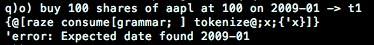
\includegraphics[scale=0.5]{internal-parse-error.jpeg}
\caption{Internal: bad date error}
\end{figure}
\begin{figure}[ht]
\centering
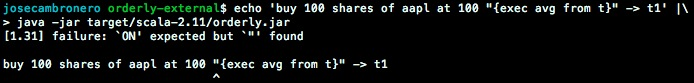
\includegraphics[scale=0.45]{external-parse-error.jpeg}
\caption{External: missing modifier keyword (if or on)}
\end{figure}
\end{frame}


\begin{frame}{Semantic Analysis}
Do: protect users from "silly" mistakes \\
In orderly: verifying that volume and price are positive \\

In reality: \\
For external: some soft type checking \\
For internal: early type checks/validation \\
Improve common sources of issues for newcomers: \\
   - exceeding local in functions ---$>$ convert those functions to use dictionaries for local variables\\
   - stackoverflow for mutually recursive functions --$>$ if tail calls, use trampolines \\
   - lack of local statically scoped vars  ---$>$ added these as function params
\end{frame}


\begin{frame}{Semantic Analysis/ Optimizations}
Interpreter: harder if chose shallow, deep embedding reifies operations to data, and that along with 
eval/parse (meta programming) can transform \\
External: pick an implementation language that allows nice rewrites: pattern matching (common in functional languages) makes life easier \\

In orderly: we can take separate insertions (order -$>$ t) and rather than obey the user, we can combine them into a
bulk insert. This can speed things up significantly \\

In aquery: AST rewrites include filter pushing, order removal, order simplification, amongst others \\

Dos: generate modular, clean rewrite rules \\
Dos: be clear on the rewrite strategy (can it be done statically, if external? if so, apply.  Can it be done by delaying until runtime to perform it better?) \\

For internal, deep interpreter: pattern matching would be nice... if someone wants to contribute that...I've started fooled around with it before, but efficient version is needed \\
\end{frame}

\begin{frame}{Code generation/Execution}
Interpreter: for deep, at this point you should hand off to an interpreting function. For shallow, you will have built a 
series of composed function calls \\

External: Generate q code to file/stdout for later execution. \\

Dos: generate intelligible code if external (ideally you should be able to read it and easily spot errors) \\
Dos: take advantage of static info, but don't be afraid to delay checks to runtime if necessary/helpful \\
Dos: Make sure to provide power users a way to provide expressions in your language that are directly carried
over to q (e.g. verbatim q code in aquery) \\
\end{frame}




\begin{frame}[allowframebreaks]
        \frametitle{References}
        \bibliographystyle{plain}
        \bibliography{bibliography.bib}
\end{frame}

\end{document}
